\subsection{Hidden Markov Models (HMM) \skript{122-131 and HMM-Skript}}

\renewcommand{\arraystretch}{1.5}
\begin{tabular}{llll}
Hidden Markov Model& $M$&&\\
Probability of transition from state $i$ to state $j$:&
$P_{ij}=P(X_{t+1}=j|X_t=i)$&&\\
Probability of emitting symbol $j$ in state $i$ :&
$O_{ij}=P(Y_{t}=s_j|X_t=i)$&&\\
Initial probability to be in state $i$:&
$\bm{\pi_i}:=P(X_1=i),i \in S$&&\\
Hidden sequence:&
 $X_t$\quad such as $X_t=\{x_1,x_2,\ldots,x_t\}$&or& $X_{t+1}=\{x_1,x_2,\ldots,x_t,x_{t+1}\}$\\
Observed sequence:&
 $Y_t$\quad ~such as $Y_t=\{y_1,y_2,\ldots,y_t\}$&or& $Y_{t+1}=\{y_1,y_2,\ldots,y_t,y_{t+1}\}$\\
Number of hidden states & $N$&&\\
Time & $1 \leq t \leq T$&&
\end{tabular}

\renewcommand{\arraystretch}{1.0}
\begin{equation}
	\bm{P}=\begin{pmatrix}
		a_{11} & a_{12} & a_{13}\\
		a_{21} & a_{22} & a_{23}\\
		a_{31} & a_{32} & a_{33}
	\end{pmatrix} \quad
	\sum\limits_j a_{ij} = 1\\ 
	\bm{O}=\begin{pmatrix}
		b_{11} & b_{12} & b_{13} & b_{14}\\
		b_{21} & b_{22} & b_{23} & b_{24}\\
		b_{31} & b_{32} & b_{33} & b_{34}\\
	\end{pmatrix} \quad
	\sum\limits_k b_{jk} = 1\\
	\bm{\pi}=\begin{pmatrix}
		\pi_1\\
		\pi_2\\
		\pi_3\\
	\end{pmatrix}\nonumber
\end{equation}

\begin{minipage}{0.3\textwidth}
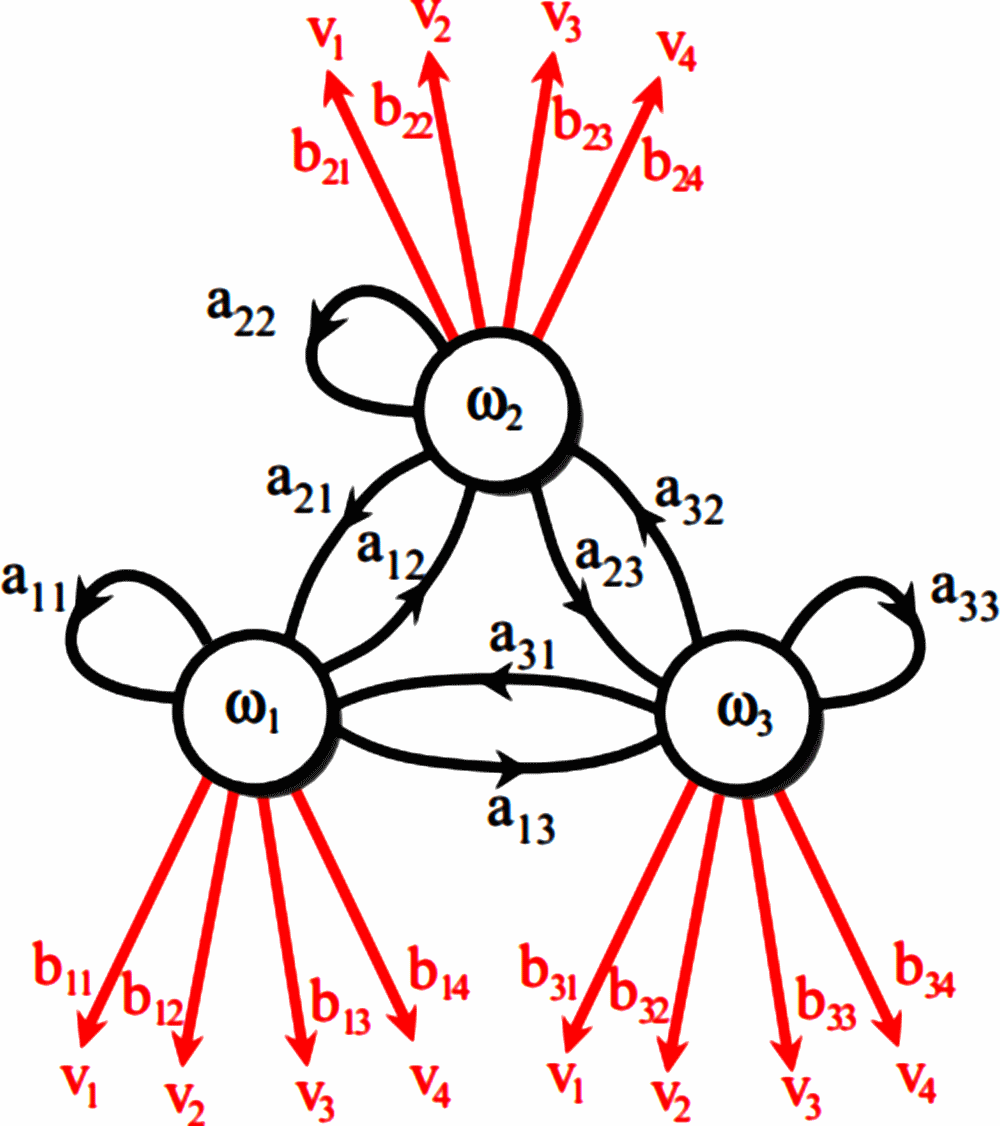
\includegraphics[width=1\linewidth]{./Content/Markov/hiddenMarkovModel.png}
\end{minipage}
\begin{minipage}{0.4\textwidth}
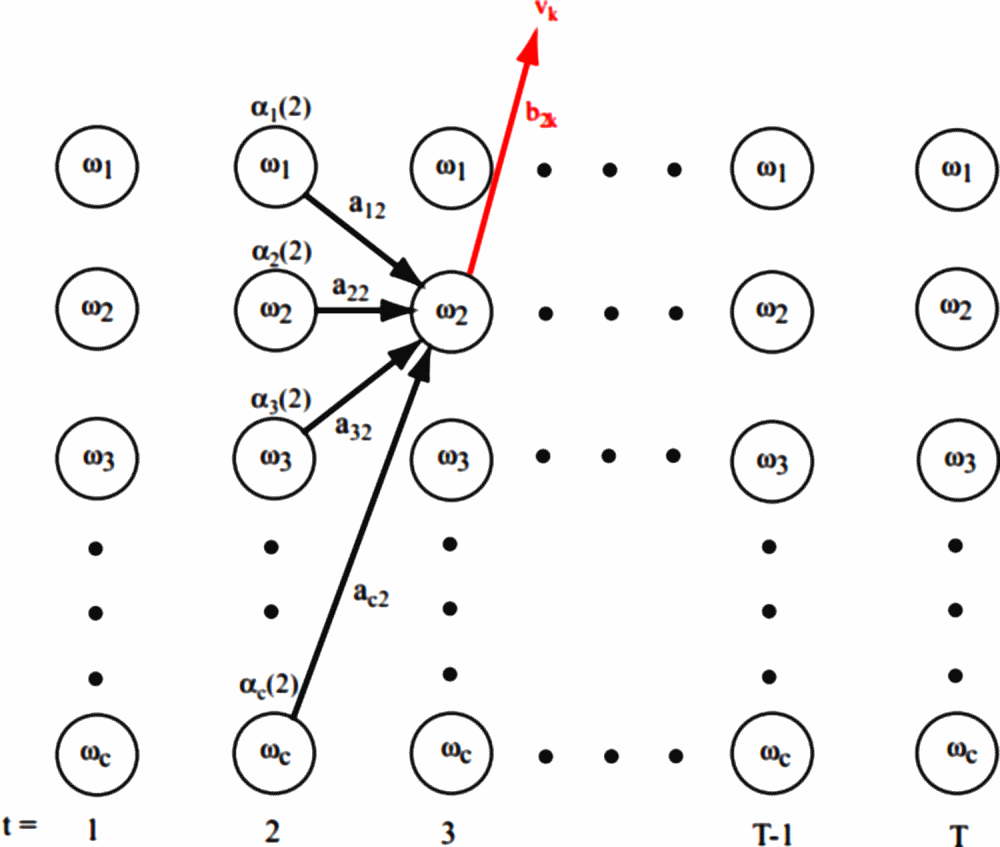
\includegraphics[width=1\linewidth]{./Content/Markov/hiddenMarkovModel2.png}
\end{minipage}
\begin{minipage}{0.3\textwidth}
  \subsection{Problems}
    \begin{liste}
      \item Evaluation problem: Determine the \em probability \em that a particular sequence of 
      visible states $\bm V_T$ was generated by \em that model\em.
      \item Decoding problem: Determine the \em most likely sequence of hidden states \em $\bm \omega^T$ that
      led to observations $\bm V_T$.
      \item Learning problem: Given the structure and training observations, \em learn the parameters \em
      $a_{ij}$ and $b_{jk}$. 
    \end{liste}
\end{minipage}
\vspace{5mm}
\hrule
\vspace{5mm}
\begin{minipage}{0.55\textwidth}
	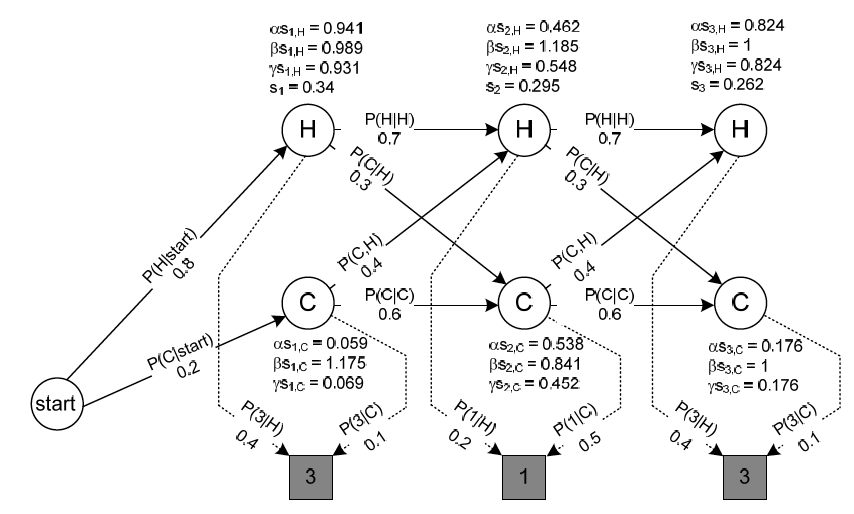
\includegraphics[width=1\linewidth]{./Content/Markov/hmm.png}
\end{minipage}
\begin{minipage}{0.44\textwidth}
	\textbf{Example:}\\
	\begin{tabular}{ll}
											&	Scaled	\\
	$\alpha_{1,H}=P(H|start) P(3|H)$	&	$\alpha S_{1,H}= \displaystyle\frac{\alpha_{1,H}}{\alpha_{1,H}+\alpha_{1,C}} $ \\
	$\alpha_{1,C}=P(C|start) P(3|C)$	&	$\alpha S_{1,C}= \displaystyle\frac{\alpha_{1,C}}{\alpha_{1,H}+\alpha_{1,C}}$ \\
	\end{tabular}
	
	$\alpha_{2,H}=\alpha_{1,H}P(H|H)P(1|H) + \alpha_{1,C}P(C|H)P(1|H)$ \\
	$\alpha_{2,C}=\alpha_{1,H}P(H|C)P(1|C) + \alpha_{1,C}P(C|C)P(1|C)$ \\
	
	$\beta_{1,H}=\beta_{2,H}P(1|H)P(H|H) + \beta_{2,C}P(1|C)P(C|H)$ \\
	$\beta_{1,C}=\beta_{2,C}P(1|C)P(C|C) + \beta_{2,H}P(1|H)P(H|C)$ \\
	
	$\gamma_{1,H}=\alpha_{1,H}\beta_{1,H}$ \\
	$\gamma_{1,C}=\alpha_{1,C}\beta_{1,C}$ \\
 
	 
	
\end{minipage}
\hrule
\vspace{5mm}

\begin{minipage}[t]{0.49\textwidth}

\subsection{Forward Algorithm (Evaluation)}
The forward algorithm can be used to find the probability of an observed sequence $Y_t$.

\begin{aufzaehlung}
	\item Initialization for states $1\leq i \leq N$ at time $t=1$:\\
	
	\vspace{-0.3cm}
	
	$\boxed{\textcolor{blue}{\alpha_1}(i)=\pi_i b_j(y_1)}$ 
	
	\item Recursion for states $1\leq j \leq N$ and time $1\leq t\leq T-1$:\\
		
	\vspace{-0.3cm}
	
  $\boxed{\textcolor{blue}{\alpha_{t+1}}(j)=b_{j}(y_{t+1}) \sum\limits_{i=1}^{N}{\textcolor{blue}{\alpha_t}(i)a_{ij}}}$
	
	\item Total probability for unscaled values\\
		
	\vspace{-0.3cm}
	
	$\boxed{P_{tot} = P(Y_t|M)=\sum\limits_{i=1}^{N}{\textcolor{blue}{\alpha_T(i)}}}$
\end{aufzaehlung}
\end{minipage}
\hfill
\begin{minipage}[t]{0.49\textwidth}
\subsection{Backward Algorithm (Evaluation)}
The backward algorithm is important for the Baum-Welch algorithm. If the target is to find the probability of an observed sequence $Y_t$, then 
the forward algorithm is sufficient. The backward algorithm starts from the last observation and goes backwards.

\begin{aufzaehlung}
	\item Initialization for $1 \leq i \leq N$ at time $t=T$:\\
	
	\vspace{-0.3cm}
	
	$\boxed{\textcolor{blue}{\beta_T}(i)=1}\to$ where $T$ is the last observation time
	\item Recursion for states $1 \leq j \leq N$ and time $2\leq t\leq T$:\\
	
	\vspace{-0.3cm}
	
	 $\boxed{\textcolor{blue}{\beta_{t-1}}(j)=\sum\limits_{i=1}^{N}{b_i(y_t)\textcolor{blue}{\beta_t}(i)a_{ji}}}$
	 \item Conditional probability for the state $x_i$:\\
	 	
	 \vspace{-0.3cm}
	 	
	 $\boxed{P(X_t=x_i|Y_t,M)=\frac{P(X_t=x_i,Y_t|M)}{P(Y_t|M)}=\frac{\textcolor{blue}{\alpha_t}(i)\textcolor{blue}{\beta_t}(i)}{P(Y_t|M)}}$
	 
\end{aufzaehlung}
\end{minipage}

\vspace{1cm}

\begin{minipage}[t]{0.49\textwidth}
\subsection{Viterbi Algorithm (Decoding)}
Be aware, this is not always the same $\alpha$ as in the forward algo (except for $\alpha_1(i)$).
\begin{aufzaehlung}
	\item Initialization for $1\leq i \leq N$:\\
	
	\vspace{-0.3cm}
	
	$\boxed{\textcolor{blue}{\alpha_1}(i)=\pi_i b_j(y_{1})}$
	\item Recursion for $1\leq t\leq T-1$ and $1\leq j \leq N$:\\
			
		\vspace{-0.3cm}
		
		$\boxed{\textcolor{blue}{\alpha_{t+1}}(j)=b_{j}(y_{t+1}) \max\limits_{i \in \{1,\ldots,N\}}{\textcolor{blue}{\alpha_t}(i)a_{ij}}}$
		
		\item Termination: (find the winner state)\\
			
		\vspace{-0.3cm}
		
		$\boxed{P(X_t|Y_t)=\max\limits_{j \in \{1,\ldots,N\}}{\textcolor{blue}{\alpha_T}(j)}}$
	\item Backtracking (All the stored way back):\\
				
		\vspace{-0.3cm}
			
		$\boxed{X_t=\arg~ \underset{j \in \{1,\ldots,N\}}{\max}~{\textcolor{blue}{\alpha_T}(j)}}$\\
		Starting from the biggest argument of $\alpha_T$ go backwards through the edges with the highest probability.
\end{aufzaehlung}	 
\end{minipage}
\hfill
\begin{minipage}[t]{0.49\textwidth}

\subsection{Baum-Welch Algorithm (Learning)}

\begin{aufzaehlung}
	\item Initialization for $1\leq i \leq N$:\\
	
	\vspace{-0.3cm}
	
	Assign arbitrary model parameters\\

	\item Iteration:\\
			
	\vspace{-0.3cm}
	
	Set $\bm{A_{kl}}$ and $\bm{B_{k}(x)}$ to a pseudocount value.\\
	
	FOR  each training data set $\bm{X}^m$:\\
	
	\qquad Forward algoritm: $\textcolor{blue}{\alpha_t}(i)$
	
	\qquad Backward algoritm: $\textcolor{blue}{\beta_t}(i)$
	
	\qquad Add contributions to $\bm{A_{kl}}$ and $\bm{B_{k}(x)}$
	
	\qquad Update $a_{ij}=\frac{A_{ij}}{\sum\limits_{k}^{}{A_{ik}}}$ and $b_k(x)=\frac{B_k(x)}{\sum\limits_{l}^{}{B_{k}(l)}}$
	
	\item Termination:\\
		
	UNTIL stop criterion reached
		
\end{aufzaehlung}	 
\end{minipage}

\subsection{Some properties}
\begin{itemize}
	\item The $\gamma$-Value: $\boxed{\gamma_t(j)=\textcolor{blue}{\alpha_t}(j)\cdot\textcolor{blue}{\beta_t}(j)}$
	\item A property of the $\gamma$-Value: is: $\boxed{\sum\limits_{j=1}^{N}{\gamma_t(j)=P_{tot}}}$ \\  
	$\to$ Example: $P_{tot}=\gamma_2(Hot)+\gamma_2(Cold)=\alpha_2(Hot)\cdot\beta_2(Hot)+\alpha_2(Cold)\cdot\beta_2(Cold)$
	\item Probability that the state was $x$ at time $t$ given the sequence $Y_t$: $\boxed{P(X_t=x|Y_t)=\frac{\textcolor{blue}{\alpha_t}(x)}{\sum\limits_{j=1}^{N}{\textcolor{blue}{\alpha_t}(j)}}}$
\end{itemize}



